\section{Results}
\label{sec:results}

Throughout, $\dNE$ is measured against \textsc{Wait} --- the segregated status quo that joins on
the attribution window --- so negative means the short join is better.

\paragraph{The join window can be collapsed.}
Writing the record \ratioSeven{} times sooner than the seven-day window it is accountable to,
and letting the teacher stand in for the conversions not yet seen, lowers $\NE$ in all
\nContrast{} cells --- every one significant --- by \collapseSevenBest{} to
\collapseSevenWorst{} (Fig.~\ref{fig:delta}). At the one-day window the same
substitution gains \collapseOneBest{} to \collapseOneWorst{}, significant in
\collapseOneSig{}.

The two windows differ by a factor of three in the mean (\collapseSevenMean{} against
\collapseOneMean{}), and the direction is the useful part: \emph{the slower the funnel, the
more collapsing its join window is worth}. This inverts the intuition --- a longer window
censors more of the label, so the teacher has more to supply --- because what dominates is the
cost of the alternative: \textsc{Wait} at $v=7$\,d trains on week-old data, and no label
accuracy compensates.

\begin{figure}[t]
\centering
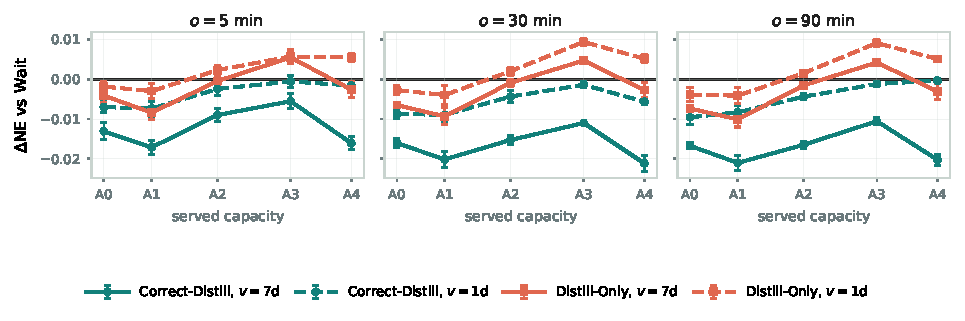
\includegraphics[width=\textwidth]{figs/delta}
\caption{$\dNE$ against \textsc{Wait}; below the line beats the segregated status quo. Colour
is the target, dash the attribution window. \textsc{Correct-Distill} is below the line
everywhere and furthest below at $v=7$\,d; \textsc{Distill-Only} crosses it between A1 and A2
at every join delay when $v=1$\,d. Bars are the standard deviation of the five per-seed
differences.}
\label{fig:delta}
\end{figure}

\paragraph{The condition: keep part of the hard label.}
The collapse above used the hybrid target; the fully soft one decides how far the result can be
pushed. At $v=1$\,d, \textsc{Distill-Only} beats
\textsc{Wait} at the two smallest capacities (\doSmall{} on average) and \emph{loses} at the
three largest (\doLarge{}), crossing over between A1 and A2 at every join delay
(Fig.~\ref{fig:delta}); all \doSig{} cells are significant, so the crossing is not noise. A purely soft target plausibly acts as a regulariser, a variance reduction a small model can
use and a larger one no longer needs~\cite{menon2021statistical}. This cuts against
convenience: a record with no hard label is the most portable object a consolidated pipeline
could ask for, and it is exactly the one that fails at the capacities worth serving. At $v=7$\,d the crossover is weaker and
non-monotone (\textsc{Distill-Only} returns to \doSevenLargest{} at A4), so we state the rule
for the one-day window and do not extrapolate it.

\paragraph{The teacher need not be live.}
Our teacher keeps learning from the matured stream, making it a service rather than an
artifact. Freezing it after causal initialisation costs \frzOne{} $\NE$ at one day and
\frzSeven{} at seven, and frozen \textsc{Correct-Distill} still beats \textsc{Wait} in
\frzSevenBeat{} of \frzSevenN{} cells at seven days: a shipped model, not a running
maturity-gated service, suffices.

\paragraph{Two anchors.}
Two anchors fix the scale. \textsc{Wait} beats \textsc{Fresh} --- the same short join with no
correction --- by \waitFreshFive{} at $o=5$ minutes, so the gap the teacher is filling is an
order of magnitude larger than the gains above, and an uncorrected short join is not an option.
\textsc{Correct-Distill} and \textsc{Ulc}~\cite{wang2023unbiased} share Eq.~\eqref{eq:hybrid}
and differ only in how the corrector is estimated; they are near-indistinguishable (mean $\dNE$ \cdUlcMean{}, \cdUlcNs{} of \nContrast{} cells
not significant at $v=1$\,d). The offline teacher does not beat the online corrector on
accuracy; the case for it is architectural (Sect.~\ref{sec:consolidation}).
